\section{Valutazione dell'esplorazione} \label{sec:valutazione_esplorazione}
Come accennato in \ref{subsubsec:expl_funct}, andare a valutare per ogni punto campionato l'esplorazione \textbf{globale} risulta estremamente costoso, implicando dei tempi di simulazione estremamente lunghi.
Inoltre, l'uso di questo approccio è poco utile; infatti dopo il movimento degli agenti nelle zone lontane dal punto campionato in esame avrò verosimilmente uno stato di esplorazione diverso, rendendo la previsione fatta su quelle celle durante la valutazione del punto ottimo poco attendibile.
A fronte di queste problematiche, durante le fasi sperimentali sono stati progettati e implementati diversi metodi per valutare localmente il livello di esplorazione di un punto, in modo che tale operazione risulti computazionalmente valida.

% metto prima il metodo finale, e poi le caratteristiche di quellli vecchi le ricollego a queste?
\subsection{Metodi sperimentali per la valutazione dell'esplorazione} \label{subsec:experimental_expl_eval}
In questa sotto-sezione si riportano i vari metodi sviluppati durante le fasi di test, ma che sono stati rimpiazzati da una versione successiva più accurata, fino ad arrivare a quello utilizzato negli esperimenti, ed esposto in \ref{subsec:expl_eval_frontier_NCC}.

\subsubsection{Simple Exploration}
Questo metodo è stato utilizzato nelle fasi iniziali per verificare la variazione di probabilità delle celle in tempi di simulazione ragionevoli. 
Esso non tiene conto del SINR per valutare la copertura di un cella, ma controlla soltanto che il suo centro sia abbastanza vicino ad un sensore.
Per ovvi motivi, tale metodo è stato rapidamente sostituito dai successivi.

\subsubsection{Local Square Interference Exploration (LSIE)}
In questa variante, si va a valutare la copertura di una cella tramite il livello di SINR calcolato nel suo centro, rendendo il requisito di copertura della cella simile a quello della copertura utente.
La novità principale è quella di non considerare tutte le celle della matrice, ma soltanto quelle che rientrano all'interno di un'area quadrata centrata nella posizione dell'agente, di lato \texttt{2$\cdot$EXPLORATION\_RADIUS} (Figura \ref{fig:esempio_LSIE}).
\begin{SCfigure}[1][h]
    \centering
    \caption[Esempio dell'area valutata con il metodo LSIE]{Esempio dell'area considerata dal metodo LSIE; si osserva come le celle presenti negli angoli dell'area siano difficilmente raggiungibili dal segnale dell'agente.}
    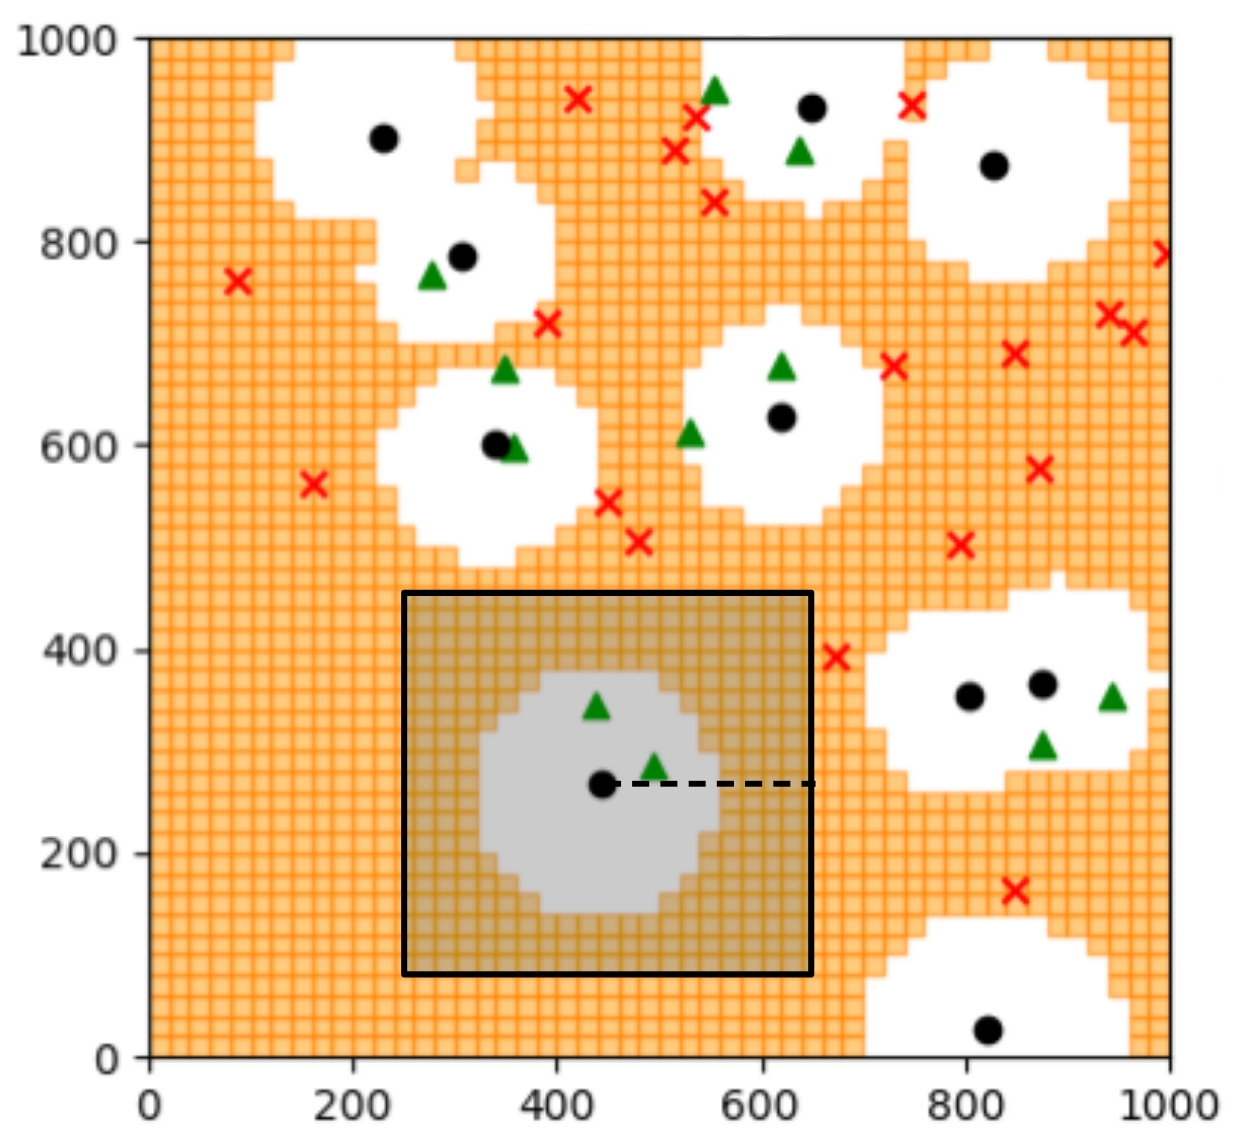
\includegraphics[width=0.5\textwidth]{img/ch3/esempio_LSIE.jpg}
    \label{fig:esempio_LSIE}
\end{SCfigure}

Inoltre si vanno a considerare soltanto le interferenze provenienti da sensori relativamente vicini all'agente, in quanto una eccessiva distanza rende il segnale d'interferenza trascurabile; questa considerazione permette di avere un minor numero di agenti nel calcolo del SINR, alleggerendo il costo computazionale.
Si osserva come la scelta del valore di \texttt{EXPLORATION\_RADIUS} sia critica, in quanto  un raggio maggiore implica una visione più approfondita dell'ambiente da parte dell'agente, comportando però una minore velocità del metodo.
\textbf{Sperimentalmente} si è osservato che ponendo \texttt{EXPLORATION\_RADIUS=200} si ha un'esplorazione completa dell'area intorno ad un punto, mantenendo un buon tempo di simulazione.
Il problema di questa variante è che, data la forma quadrata dell'area, si andranno a considerare anche le celle negli angoli, che molto probabilmente non saranno mai coperte dal segnale dell'agente (Figura \ref{fig:esempio_LSIE}).


\subsubsection{Local Circle Interference Exploration (LCIE)}
Rispetto al metodo precedente questa variante modifica la forma dell'area osservata, passando dall'utilizzo di un'area quadrata ad una circolare, rimuovendo quindi le celle che prima si trovavano negli angoli; questo porta ad un'ulteriore aumento di velocità del processo di valutazione, essendosi ridotto il numero di celle da osservare.
\begin{figure}[h]
    \centering
    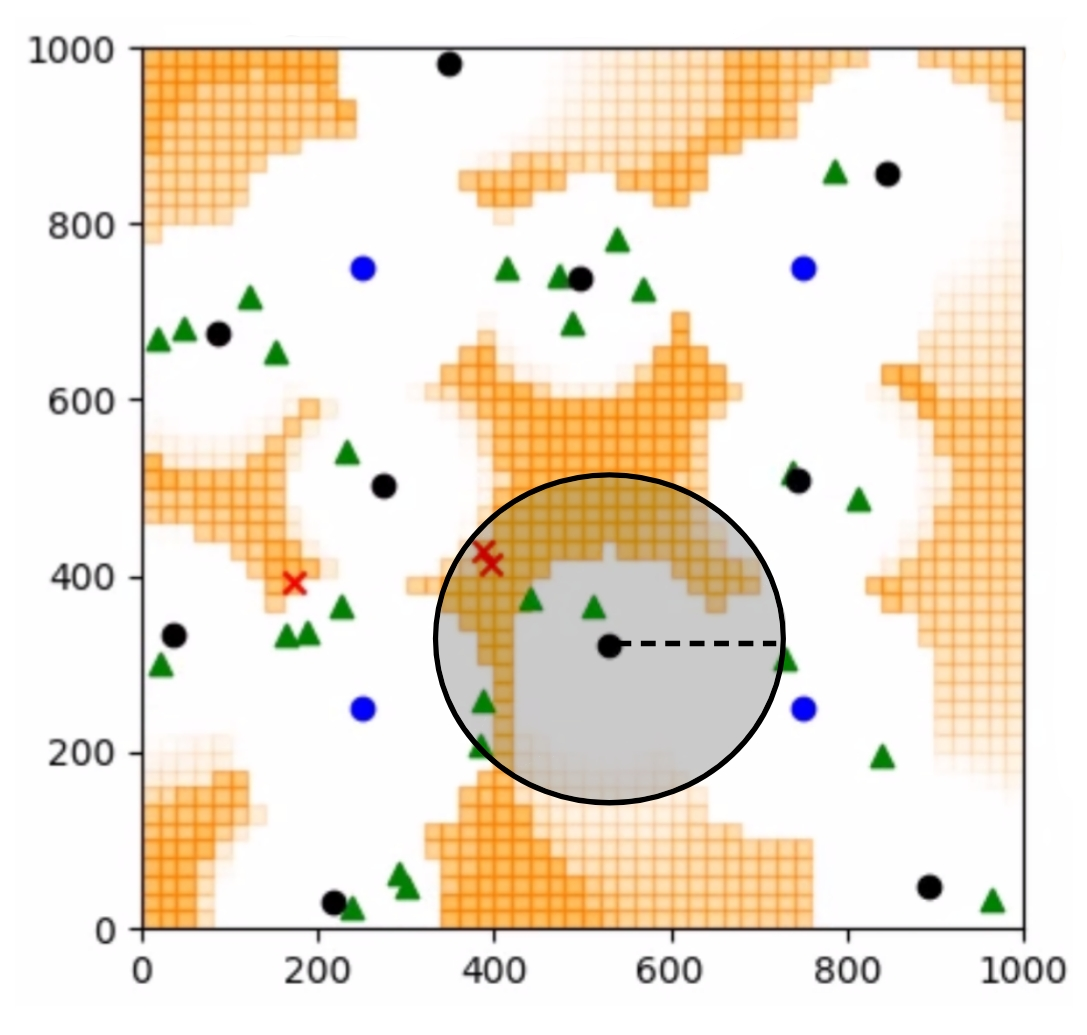
\includegraphics[width=0.5\textwidth]{img/ch3/esempio_LCIE.jpg}
    \caption[Esempio dell'area valutata con il metodo LCIE]{Esempio di area considerata dal metodo LCIE.}
    \label{fig:esempio_LCIE}
\end{figure}

\subsubsection{Local Square Interference Exploration, Neighbour Cell Control (LSIENCC)}
Implementata prima della \textit{Local Circle Interference Exploration}, questo metodo aggiunge una predizione sul livello di copertura di alcune celle quando sono soddisfatte alcune condizioni.
Tale predizione si basa sull'osservazione che, se il SINR calcolato in una cella è abbastanza alto, allora con molta probabilità anche quello delle celle adiacenti supererà la soglia richiesta.
Seguendo tale euristica, è possibile ridurre drasticamente i tempi di valutazione dell'esplorazione di quegli agenti isolati rispetto al resto della rete: infatti, la distanza da gli altri agenti fa sì che il livello di SINR rimanga abbastanza uniforme lungo l'area.
\subsection{Valutazione dell'esplorazione tramite frontiera con controllo delle celle adiacenti} \label{subsec:expl_eval_frontier_NCC}
Il metodo riportato in questa sotto-sezione è quello che verrà usato nelle simulazioni esposte nel Capitolo \ref{ch4:simulazioni}.
Esso è la combinazione delle varianti \textit{LCIE} e \textit{LSIENCC}, esposte nella sotto-sezione precedente; tale metodo include dunque i vantaggi di avere una regione da valutare il più ridotta possibile, senza però rinunciare alla precisione della stima, e di poter predire il livello di copertura di alcune celle, senza doverne calcolare esplicitamente il valore.

% da ricontrollare
I passaggi principali in cui l'algoritmo si articola sono i seguenti:
\begin{enumerate}[wide]


\item
Per prima cosa, il metodo seleziona quelle celle che rientrano nell'area da valutare, inserendo le informazioni rilevanti (posizione del centro e probabilità) in una struttura dati simile ad una matrice, ma con lunghezza delle righe variabile (Snippet \ref{snip:init_expl_eval}).
Inoltre, identifica gli agenti abbastanza vicini al punto campionato.
\lstinputlisting[
language=Python 
, label={snip:init_expl_eval}
, caption={Inizializzazione del metodo LCIENCC.}
, frame=tb
, float = ht
, belowcaptionskip=3mm
]{code/init_expl_eval_method.py}


\item
Successivamente, per ogni cella inclusa, calcola il SINR di ciascun agente precedentemente selezionato.
Dal calcolo del SINR vengono escluse quelle celle aventi $P_k=0$,  in quanto sono già coperte, e non apporterebbero nessun contributo all'esplorazione (Snippet \ref{snip:core_expl_eval}).
Se il livello di SINR di una cella supera una certa soglia \texttt{NEIGHBOUR\_SINR\_THRESHOLD}, la cella sovrastante e quella a destra (quella sotto e quella a sinistra sono state già esaminate) vengono inserite in \texttt{already\_checked\_cells}, ossia una lista che permette di escludere tali celle dalla valutazione del livello di SINR.
Prima di tale inserimento, viene fatta una serie di controlli per escludere quelle celle che eccedono l'aera di valutazione, e per evitare di etichettare come coperta una cella avente probabilità zero. 
\lstinputlisting[
language=Python 
, label={snip:core_expl_eval}
, caption={Calcolo della copertura nel metodo LCIENCC.}
, frame=tb
, float = p
, belowcaptionskip=3mm
]{code/core_expl_eval_method.py}


\item
Infine si calcola il livello di esplorazione, basandosi sulla matrice che associa a ciascuna cella il valore di SINR di ogni agente. (Snippet \ref{snip:final_expl_eval}).
\lstinputlisting[
language=Python 
, label={snip:final_expl_eval}
, caption={Valutazione dell'esplorazione nel metodo LCIENCC.}
, frame=tb
, float = h
, belowcaptionskip=3mm
]{code/final_expl_eval_method.py}


\end{enumerate}